The final states to which the heavy photon can decay into is related to the model of the dark sector, and corresponding dark matter mass $m_{\chi}$, one is considering. For a heavy photon that is heavier than $m_{\chi}$, then the heavy photon may decay into completely invisible states or a mixture of invisible states and SM states. For the scenario that the heavy photon decays to completely invisible states, the experiment will perform a missing mass or missing momentum measurement in order to identify the heavy photon signal. Here, we focus solely on the scenario of a heavy photon that decays visibly to SM particles (this also implies that the heavy photon is lighter than the dark matter mass). Due to the mechanism of kinetic mixing, the production of the heavy photon is similar to that of a photon radiating from an electron although at a suppressed rate proportional to the coupling $\epsilon^2$. 

\subsection{Decay signature}
The branching ratio of the heavy photon is derived from the ratios of different final state measurements of $e+e-\rightarrow$ hadrons at various center-of-mass energies~\cite{weiner}. In the mass regime that HPS explores, the heavy photon can be expected to primarily decay to $e+e-$ pairs as shown in Figure~\ref{Figure:br}. 

\begin{figure}[H]
  \centering
      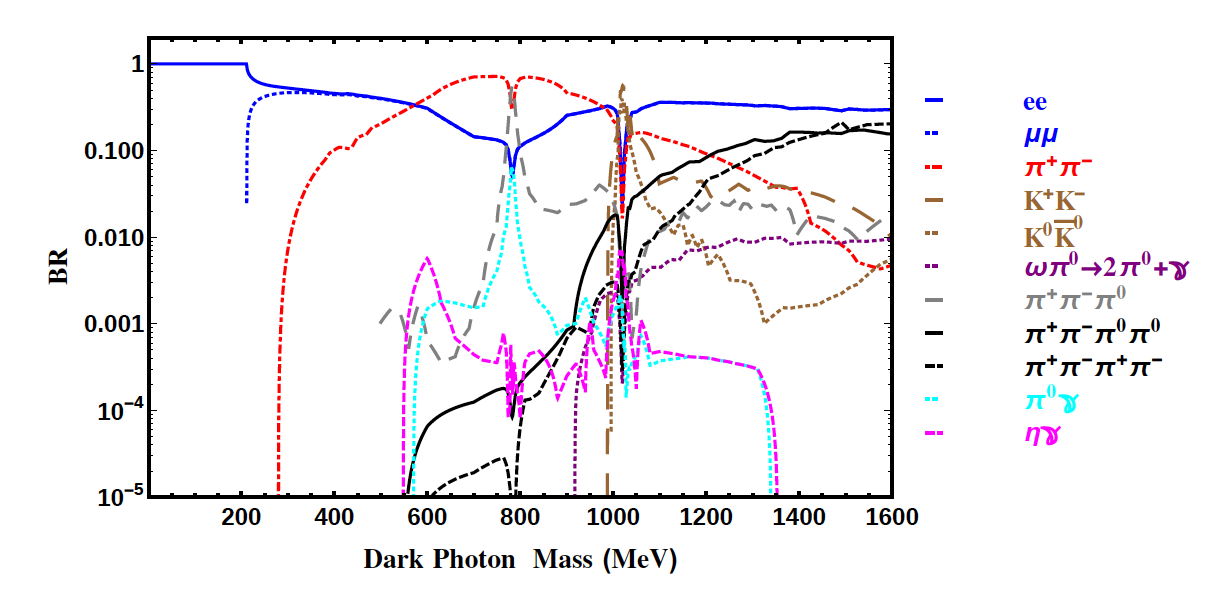
\includegraphics[width=0.9\textwidth]{pics/motivation/branchingRatio.png}
  \caption[The branching ratios for heavy photon decays]{The branching ratios for heavy photons of various masses.~\cite{weiner}}
  \label{Figure:br}
\end{figure}

HPS searches for heavy photons of masses 20 to 100~MeV/c$^2$. As shown in Figure~\ref{Figure:br}, at heavy photon masses above 200~MeV/c$^2$, the branching ratio for decays to $e+e-$ begins to decrease sharply and the turn on for decays to $\mu+\mu-$ becomes significant. \\
\indent Assuming that the heavy photon only decays to SM final states, the proper lifetime of the A$^{\prime}$ neglecting phase space corrections is described by Equation~\eqref{eq:propLife} where $N_{eff}$ is the number of available decay states ($=1$ at $m_{A^{\prime}}<2m_{\mu}$).~\cite{toro} 

\begin{eqnarray}
	\label{eq:propLife}
	c\tau &=& \dfrac{1}{\Gamma}\simeq \dfrac{3}{N_{eff}m_{A^{\prime}}\alpha\epsilon^2}\\
	&\simeq & \dfrac{0.8\textsf{ cm}}{N_{eff}}\Big({\dfrac{10^{-4}}{\epsilon}}\Big)^2\Big(\dfrac{100\textsf{ MeV}}{m_{A^{\prime}}}\Big)\\
\end{eqnarray}

As shown in Equation~\eqref{eq:propLife}, the lifetime is inversely related to the coupling $\epsilon^2$. For small couplings, the heavy photon will travel a measurable distance after production before decaying. The decay length is described by Equation~\eqref{eq:decayL}.

\begin{eqnarray}
	\label{eq:decayL}
	l_0 &\equiv &\gamma c \tau \\
	&\simeq & \dfrac{0.8\textsf{ cm}}{N_{eff}}\Big(\dfrac{E_{beam}}{10\textsf{ GeV}}\Big)\Big({\dfrac{10^{-4}}{\epsilon}}\Big)^2\Big(\dfrac{100\textsf{ MeV}}{m_{A^{\prime}}}\Big)^2\\
\end{eqnarray}

In Equation~\eqref{eq:decayL}, $E_{beam}$ refers to the incident beam energy of the electron. The rate of A$^{\prime}$ production is controlled by $\alpha^3\epsilon^2/m_{A^{\prime}}^2$ and is suppressed relative to ordinary bremsstrahlung by a factor of $\epsilon^2m_{e-}^2/m_{A^{\prime}}^2$. The ratio of the fully differential production cross sections for the heavy photon relative to the production of a virtual photon are described in Equation~\eqref{eq:production}.

\begin{equation}
	\label{eq:production}
	\dfrac{d\sigma(e-Z(A^{\prime}Z\rightarrow l+l-))}{d\sigma(e-Z(\gamma^{\ast}Z\rightarrow l+l-))} = \Big(\dfrac{3\pi\epsilon^2}{2N_{eff}\alpha}\Big) \Big(\dfrac{m_{A^{\prime}}}{\delta m_{A^{\prime}}}\Big)
\end{equation}

In Equation~\eqref{eq:production}, this ratio represents the maximum signal to background that can be achieved in an experiment. The heavy photon is produced at very forward, small angles and carries nearly all of the beam energy. \\
\indent Some of the formalism thus far has hinted at the production of heavy photons through bremsstrahlung-like processes of an incident electron beam on a fixed target (as in the HPS setup). However, there are other experimental processes that search for the heavy photon through other means of production. These processes include annihilations of $e+e-$ particles in collider experiments. Collider experiments are more often used for looking for heavy photons that may have invisible decay modes using missing mass measurements. Looking for heavy photons produced in meson decay channels such as Dalitz decays ($\pi^0, \eta, \eta^{\prime}\rightarrow \gamma A^{\prime}$) and rare meson decay channels ($K\rightarrow\pi A^{\prime} $, $\phi\rightarrow\eta A^{\prime}$, and $D^{\ast}\rightarrow D^{0}A^{\prime}$) are another production mechanism that has been used at both colliders and fixed target-type experiments. Drell-Yan ($q\bar{q}\rightarrow A^{\prime}$) experiments are more common at proton fixed target and hadron collider experiments. 

\subsection{Heavy photon search strategies}

The strategies for searching for heavy photons are typically a bump hunt on the visible final state particles, a bump hunt on the missing mass (assumes that the heavy photon is not always decaying visibly), or a detached vertex search for heavy photons with small couplings. \\
\indent The bump hunt search on visible decays looks for a resonance on the reconstructed invariant mass spectrum of the final state pairs. The strongest limits from these experiments come from the NA 48/2, A1, and BaBar experiments ruling out most of the parameter space with couplings larger than $10^{-3}$. The NA-48/2 experiment at the CERN HPS collects large samples of kaons and searches for a heavy photon produced in these meson decay channels~\cite{NA48}. The A1 experiment reconstructed $e+e-$ pairs in the Mainz Microtron spectrometers~\cite{A1} and significantly ruled out the heavy photon as a explanation to resolve the muon $g-2$ anomaly. Bump hunt searches can also set limits on large heavy photons with large couplings by searching the missing mass spectrum for a resonance. BaBar, an experiment at the Stanford Linear Accelerator (SLAC) $e+e-$ collider, set limits by searching for the A$^{\prime}$ in missing mass around the $\Upsilon(2S)$, $\Upsilon(3S)$, and $\Upsilon(4S)$ resonances. \\
\indent The bump hunt searches are complemented by the beam dump searches that look for heavy photons with long decay lengths. The beam dump experiments E141 and E137 at SLAC, E774 at Fermilab, and one at Orsay~\cite{OrsayBD} were originally run to look for MeV-mass axion-type particles from electron beam dumps.~\cite{limitsBD} The results of these experiments were later re-interpreted to set limits on heavy photons with small masses and longer decay lengths. \\
